\chapter{Implementation}
\label{pass}m
The transformation of normal code into my balanced form happens automatically inside the compiler.
This requires no additional considerations of the programmer, while still providing increased robustness.
My thesis is intended as a proof of concept and as such does not balance all variables in the code.
It balances only variables on the stack, including function parameters, return values, literals and local variables.
I chose the stack as it provides a clean cut with little ambiguity for the programmer, while still balancing enough to decrease variance in \hammingw{}s by a measurable amount.
\Cref{fig:implementation} shows all candidates for balancing, as well as their relationship.
If one candidate has their value set by another (e.g. result of binary operators being stored in variables), then this introduces a dependency for this balancing.
These dependencies are shown as arrows in \Cref{fig:implementation}.
Memory locations (registers, heap memory, etc.) are balanced iff all values stored in them are balanced.

\begin{figure}[h]
  \centering
  \tikzbox{diagram-implemented.tex}
  \caption{The balancing status of my thesis project}
  \label{fig:implementation}
\end{figure}

\section{\llvm{}}
\label{llvm}
The \llvm{} compiler infrastructure project\cite{lattner2010llvm} contains a number of sub-projects, but it is mostly known for being an extremely versatile compiler.
It works by using an intermediate representation (\ir{}) specifically designed to be source and target independent, while allowing for easy automatic optimization.
As most of the work in a compiler goes into the so-called optimization passes.
This design makes the bulk of the work applicable to all languages.
A language can be added to \llvm{} by writing a frontend, translating source code to \ir{}.
The translation from \ir{} to machine code for the target architecture is then done by backends, which can also easily be added.
\Cref{fig:llvm} sketches this architecture.

\begin{figure}[h]
  \centering
  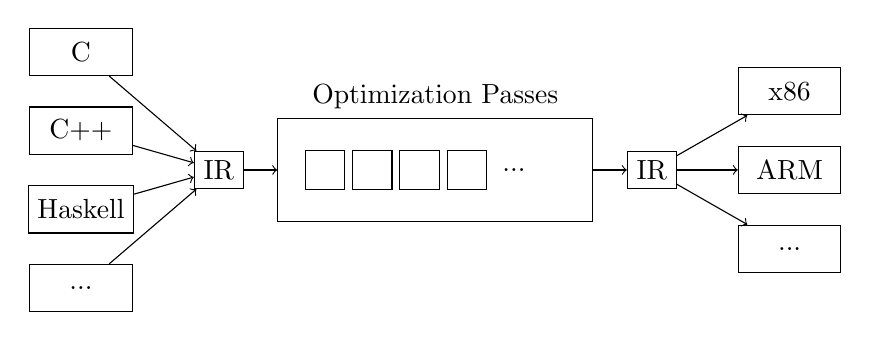
\begin{tikzpicture}
    \node[draw, minimum width=1.3cm, minimum height=0.6cm] at (-2.5,1.5) (C) {C};
    \node[draw, minimum width=1.3cm, minimum height=0.6cm] at (-2.5,0.5) (C++) {C++};
    \node[draw, minimum width=1.3cm, minimum height=0.6cm] at (-2.5, -0.5) (Haskell) {Haskell};
    \node[draw, minimum width=1.3cm, minimum height=0.6cm] at (-2.5, -1.5) (otherl) {...};
    \node[draw] at (-0.75, 0) (irl) {IR};
    
    \node[draw, label=Optimization Passes, minimum width=4cm, minimum height=1.3cm] at (2,0) (optimization) {};
    \node[draw, minimum size=0.5cm] at (0.6,0) {};
    \node[draw, minimum size=0.5cm] at (1.2,0) {};
    \node[draw, minimum size=0.5cm] at (1.8,0) {};
    \node[draw, minimum size=0.5cm] at (2.4,0) {};
    \node at (3.0, 0) {...};

    \node[draw] at (4.75, 0) (irr) {IR};
    \node[draw, minimum width=1.3cm, minimum height=0.6cm] at (6.5,1) (x86) {x86};
    \node[draw, minimum width=1.3cm, minimum height=0.6cm] at (6.5,0) (arm) {ARM};
    \node[draw, minimum width=1.3cm, minimum height=0.6cm] at (6.5,-1) (otherr) {...};

    \draw[->] (C) -- (irl);
    \draw[->] (C++) -- (irl);
    \draw[->] (Haskell) -- (irl);
    \draw[->] (otherl) -- (irl);

    \draw[->] (irl) -- (optimization);
    \draw[->] (optimization) -- (irr);

    \draw[->] (irr) -- (x86);
    \draw[->] (irr) -- (arm);
    \draw[->] (irr) -- (otherr);
  \end{tikzpicture}
  \caption{The general architecture of the \llvm{} compiler}
  \label{fig:llvm}
\end{figure}

The optimization passes at the core of \llvm{} take \ir{} as input and return it as output.
As such, optimization passes for \ir{} are immediately usable for every language and every platform that is compatible with \llvm{}.
This means implementing my balancing pass for the \llvm{} toolchain makes it very widely usable.
For this reason, and because of the powerful analysis enabled by \llvm{}'s well defined IR language, \llvm{} was chosen for my thesis.

\section{Balancing Pass}
The balancing pass stores balanced values 32 bit integers instead of regular 8 bit, and then uses my balanced arithmetic operators instead of the normal operators.
While this alone is fairly simple, it causes type mismatches for interactions between balanced and unbalanced memory.
These then need to be fixed.

Changing the arithmetic also has some implications on comparison operators.
All transformations in the order they are applied are as follows:
\begin{enumerate}
\item Change the type of all 8 bit integers (\lli8) to 32 bit integers (\lli32)
\item Balance constant initializers
\item Balance results of load operations if necessary
\item Unbalance values before store if necessary
\item Use balanced arithmetic operations instead of regular operators
\item Fix comparison directions
\item Fix type issues that arise in the instructions that have not been replaced
\end{enumerate}

The \llvm{} C++ API provides an iterator over all instructions in a function.
My pass uses this to go over all instructions, and transforms the current instruction if necessary.
This is usually done by generating a new \ir{} instruction and replacing references to the old instruction with it.

A special case are function parameters.
As these cannot be changed for an existing function, the first step in my balancing pass is to clone the original functions with changed parameter and return types.

\subsection{Cloning Functions}
Cloning functions is done in two parts.
First the prototype for the new function is created.
During this creation the pass goes through all parameter and changes their types from \lli8 to \lli32.
The same is done for the return type.
This gives me a skeleton for the balanced function, which is inserted into the module, making it accessible in the future.
All new functions are given a unique name, specifically the old name prepended with \texttt{balanced\_}.
This naming is important as it allows me to detect already balanced functions before cloning them.
It is also required to adjust the target of function calls.

The content of the original function is then copied using a helper in the \llvm{} API called \emph{CloneFunctionInto}.
Without any additional parameters, the copied instructions will still reference function parameters of the original function, will result in broken code in the new function.
To avoid this I use a so-called \emph{Value Mapper} to replace the old parameters with the new ones everywhere they are referenced.
This change alone would cause type mismatches and generates code that does not compile, but the other steps of my pass fix these problems.

\subsection{Balancing Allocations}
In order to declare and use local variables in \ir{} the memory for them first has to be allocated using the \emph{alloca} instruction.
Even function parameters are not used directly but first copied into memory explicitly allocated for this function.
Note that even though the naming is similar to C's \emph{malloc} call, the memory for \emph{alloca} is on the stack in this case.

The \emph{alloca} instruction takes the type to be allocated as parameter, and returns a pointer to that type.
This means that for balancing all the pass has to do is replace the \emph{alloca} for \lli8 with one for \lli32.
Allocations for local arrays work the same way, the pass just needs to extract the dimensions from the old allocation.

\subsection{Balancing Stores}
It can happen that the target code tries to store a balanced variable (\lli32) into an unbalanced pointer (\lli8).
In this case the pass unbalances the variable in a temporary before storing it.

While this does cause information leakage and a reduction in robustness, such a case can be avoided fairly easily.
As only global memory is unbalanced, this does not happen when the program stores all values on the stack.

\subsection{Balancing Loads}
Balancing loads is a mirror case of balancing stores.
When loading from an unbalanced pointer into a balanced variable, the pass first loads into an unbalanced temporary and then balances the value before storing it in the local variable.

%% \subsection{Balancing ZExts}
%% \emph{ZExt} stands for zero extend, and it is an instruction used to promote integer types to larger bit sizes.
%% While my pass is meant to balance code that uses \emph{only 8 bit integers}, I needed to balance \emph{ZExts} for compatibilty reasons during development and have left the balancing procedure in the code.

%% When zero extending from 8 to 32 bit, the pass replaces the instruction with a call to my balance function.
%% When extending from 32 to 64 bit it unbalances the value first and then zero extends to the target type.

\subsection{Balancing Binary Operations}
I implemented the balanced operations described in \Cref{operations} in C, each as an individual function.
In order to balance binary operations they need to be replaced by calls to these new functions.
As all binary operations are represented by the same instruction in the \llvm{} API, the pass needs to examine the \emph{opcode} of the instruction.
Based on that it decides which function call to generate.

For most operations the balanced operation is a direct implementation of the respective steps in \Cref{theory}.
Division, and remainder however are implemented by repeated addition/subtraction.
As an example, \Cref{lst:sdiv} shows the balanced function for the \texttt{sdiv} (signed division) operation in \ir{}.

\begin{lstlisting}[language=C, caption=Balanced sdiv, label=lst:sdiv]
int balanced_sdiv(int lhs, int rhs) {
  uint32_t ret = 0x00ff0000;

  uint8_t negative = 0;
  if(rhs & 0x00000080){
    negative = 1;
    rhs = balanced_negative(rhs);
  }


  while (lhs <= rhs) { //~x <= ~y iff x >= y
    lhs = balanced_sub(lhs, rhs);
    ret = balanced_add(ret, 0x00fe0001);
  }

  if(negative)
    return balanced_negative(ret);
  else
    return ret;
}
\end{lstlisting}

The semantics, especially the handling of negative values are made to be consistent with the semantics of \llvm{}.

\subsection{Balancing Pointer Arithmetic}
Balanced values cannot be used for array indexing directly.
Therefore, whenever a balanced variable is used as index for an array access it is unbalanced before use.
All array accesses use the \emph{getelementptr} instruction in \ir{}, so this is easy to catch.

\subsection{Balancing Compares}
In both of my balancing schemes the inverse occupies the more significant bits than the value itself.
This changes the direction of comparison operations, meaning \texttt{<} becomes \texttt{>}, and \texttt{>=} becomes \texttt{<=}.

\section{Building the Optimization Pass}
\label{buildpass}
The compiler pass is built using CMake as that makes loading the required parts of \llvm{} very easy.
\Cref{lst:cmakelists} shows the \emph{CMakeLists.txt} for my balancing pass.
The code is based on the template repository provided in \cite{sampson2015llvm}.

\lstinputlisting[caption=CMake configuration for my balancing pass, label=lst:cmakelists, language=CMake]{\project/passes/CMakeLists.txt}

It uses the \emph{find\_package} function of CMake, which sets the locations for definitions, header files, and link directories.
All these are needed to build my pass.
The pass itself is then built as a \emph{MODULE} library, which tells CMake to build a shared library that can be dynamically loaded at runtime by the optimizer.
As the pass is loaded by the optimizer, which is built without run-time type information (RTTI), the pass needs to be built without RTTI as well.

This configuration then builds a file called \texttt{libPasses.so}.
During the compilation of my test code (\Cref{buildtest}) I can then load this library as a plugin for the \llvm{} optimizer.
